\documentclass[10pt,twocolumn]{article}
\usepackage{two-row-acad-cv}

\usepackage[spanish]{babel} % OJO: Ajustar según idioma 
\usepackage[utf8]{inputenx}
\usepackage[T1]{fontenc}


\colorlet{cvthemecolour}{black}
%------------------------------------------------------------
% put in another colour instead of cyan to change the colour
%------------------------------------------------------------
\colorlet{cvcolour}{cyan}


\begin{document}

% -----------------------------------------------------------
% the NAME
% -----------------------------------------------------------
\nametag{Jack}{Sparrow}
\headerrule{cvcolour}{0.6cm}

% -----------------------------------------------------------
% The PHOTO and INFO BOX
% -----------------------------------------------------------
\fbox{
\begin{minipage}[t]{0.22\textwidth}
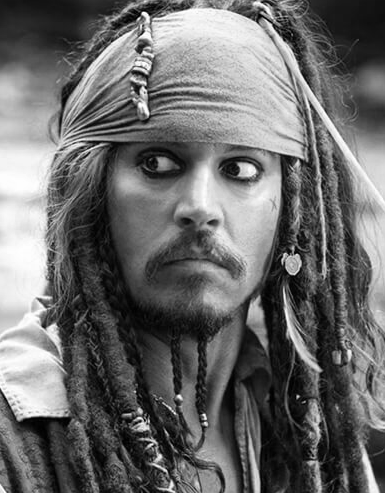
\includegraphics[valign=t,width=\textwidth]{jack-bw.png}
\end{minipage}\hspace{1em}\hfill
\begin{minipage}[t]{0.21\textwidth}
\vspace{1em}


\begin{tabular}{r|>{\footnotesize}p{0.65\textwidth}}
    \faPhone & 0043/800 010 100 \\
    \faHome & Address Line \\
    \faMapMarker & Town, Country \\
    \faAt & \texttt{jack@sparrow.com} \\
    \faLaptop & \texttt{www.sparrow.com}
\end{tabular}
\end{minipage}
}
% -----------------------------------------------------------

\vspace{2em}


\subsection{Secondary Education}
\begin{tabular}{>{\itshape}r|l}
    2018 & Certificate \\
    1990 & Education Certificate \\
    2018 & Certificate Certificate\\
    1990 & Education
\end{tabular}

\cvrule{black}{2pt}

\subsection{Secondary Education}
\begin{tabular}{>{\itshape}r|l}
    2018 & Certificate \\
    1990 & Education Certificate \\
    2018 & Certificate Certificate\\
    1990 & Education
\end{tabular}

\vspace{1em}

\subsection{Tertiary Education}
\begin{tabular}{>{\itshape}r|l}
    2018 & Certificate \\
    1990 & Education Certificate \\
    2018 & Certificate Certificate\\
    1990 & Education
\end{tabular}

\cvrule{black}{2pt}

\subsection{DEGREES}
\begin{tabular}{r p{0.8\textwidth}}
    \cvdegree{1710}{Captain}{Certified}{Tortuga Uni \color{cvcolour}}{}{disney.png} \\
    \cvdegree{1715}{Bucaneering}{M.A.}{London \color{cvcolour}}{test}{medal.jpeg} \\
    \cvdegree{1720}{Bucaneering}{B.A.}{London \color{cvcolour}}{}{medal.jpeg}
\end{tabular}


\cvrule{black}{2pt}

\begin{sansserif}
Jack \kursiv{Sparrow} is the \emph{King} of \emph{Pirates}. And a \kursiv{captain}. Open for new challenges. Lorem ipsum dolor sit amet. Lorem ipsum dolor sit amet. Lorem ipsum dolor sit amet. Lorem ipsum dolor sit amet. Lorem ipsum \kursiv{He likes rum, mosty.} sit amet. Lorem ipsum dolor sit amet. Lorem ipsum dolor sit amet. Lorem ipsum dolor sit amet.
\end{sansserif}

\cvrule{black}{2pt}


\subsection{PUBLICATIONS}
\begin{tabular}{>{\bfseries}r >{\footnotesize}p{0.4\textwidth}}
    1729\hspace{-0.5em} & \emph{How I almost got killed by Lady Swan}, in: Barbossa (ed.): \emph{Proceedings of the Pirate's Conference}, Tortuga Printing Press. \\
    1720\hspace{-0.5em} & ``Privateering for Beginners'', in: \emph{The Pragmatic Pirate} (1/1720).\\
    1729\hspace{-0.5em} & \emph{How I almost got killed by Lady Swan}, in: Barbossa (ed.): \emph{Proceedings of the Pirate's Conference}, Tortuga Printing Press. \\
    1720\hspace{-0.5em} & ``Privateering for Beginners'', in: \emph{The Pragmatic Pirate} (1/1720).
\end{tabular}

\cvrule{black}{2pt}

\subsection{PUBLICATIONS}
\begin{tabular}{>{\footnotesize\bfseries}r>{\footnotesize}p{0.4\textwidth}}
    \brackdate{1729} & \emph{How I almost got killed by Lady Swan}, in: Barbossa (ed.): \emph{Proceedings of the Pirate's Conference}, Tortuga Printing Press. \\
    \brackdate{1720} & ``Privateering for Beginners'', in: \emph{The Pragmatic Pirate} (1/1720).\\
    \brackdate{1729} & \emph{How I almost got killed by Lady Swan}, in: Barbossa (ed.): \emph{Proceedings of the Pirate's Conference}, Tortuga Printing Press. \\
    \brackdate{1720} & ``Privateering for Beginners'', in: \emph{The Pragmatic Pirate} (1/1720).
\end{tabular}

\cvrule{black}{2pt}

\subsection{PUBLICATIONS}
\begin{tabular}{>{\bfseries}r>{\footnotesize}p{0.4\textwidth}}
    \brackdate{1729} & \emph{How I almost got killed by Lady Swan}, in: Barbossa (ed.): \emph{Proceedings of the Pirate's Conference}, Tortuga Printing Press. \\
    \brackdate{1720} & ``Privateering for Beginners'', in: \emph{The Pragmatic Pirate} (1/1720).\\
    \brackdate{1729} & \emph{How I almost got killed by Lady Swan}, in: Barbossa (ed.): \emph{Proceedings of the Pirate's Conference}, Tortuga Printing Press. \\
    \brackdate{1720} & ``Privateering for Beginners'', in: \emph{The Pragmatic Pirate} (1/1720).
\end{tabular}

\cvrule{black}{2pt}

\subsection{Publications}
\begin{enumerate}[{label=[\arabic{*}]},noitemsep]
    \item \emph{How I almost got killed by Lady Swan}, in: Barbossa (ed.): \emph{Proceedings of the Pirate's Conference}, Tortuga Printing Press, 1729.
    \item ``Privateering for Beginners'', in: \emph{The Pragmatic Pirate} (1/1720).
    \item \emph{How I almost got killed by Lady Swan}, in: Barbossa (ed.): \emph{Proceedings of the Pirate's Conference}, Tortuga Printing Press, 1729.
    \item ``Privateering for Beginners'', in: \emph{The Pragmatic Pirate} (1/1720).
\end{enumerate}

\cvrule{black}{2pt}

\subsection{PUBLICATIONS}

\pubdate{1729}\emph{How I almost got killed by Lady Swan}, in: Barbossa (ed.): \emph{Proceedings of the Pirate's Conference}, Tortuga Printing Press.

\pubdate{1730}\emph{How I almost got killed by Lady Swan}, in: Barbossa (ed.): \emph{Proceedings of the Pirate's Conference}, Tortuga Printing Press.



\cvrule{black}{2pt}


\subsection{WORK EXPERIENCE}
\begin{tabular}{r| p{0.7\textwidth}}
    \cvevent{2018--2021}{Captain of the Black Pearl}{Lead}{East Indies \color{cvcolour}}{Finally got the goddamn ship back.}{disney.png} \\
    \cvevent{2019}{Freelance Pirate}{Bucaneering}{Tortuga \color{cvcolour}}{This and that. The usual, aye?}{medal.jpeg} \\
    \cvevent{2016--2017}{Captain of the Black Pearl}{Lead}{Tortuga \color{cvcolour}}{Found a secret treasure, lost the ship.}{medal.jpeg}
\end{tabular}


\cvrule{black}{2pt}

\subsection{INTERNSHIPS}
\begin{tabular}{r| p{0.7\textwidth}}
    \cvevent{2018--2021}{Captain of the Black Pearl}{Lead}{East Indies \color{cvcolour}}{Finally got the goddamn ship back.}{disney.png} \\
    \cvevent{2019}{Freelance Pirate}{Bucaneering}{Tortuga \color{cvcolour}}{This and that. The usual, aye?}{medal.jpeg} \\
    \cvevent{2016--2017}{Captain of the Black Pearl}{Lead}{Tortuga \color{cvcolour}}{Found a secret treasure, lost the ship.}{medal.jpeg}
\end{tabular}

\cvrule{black}{2pt}


\subsection{Teaching Experience}
\begin{tabular}{r| p{0.7\textwidth}}
    \cvevent{2018--2021}{Captain of the Black Pearl}{Lead}{East Indies \color{cvcolour}}{Finally got the goddamn ship back.}{disney.png} \\
    \cvevent{2019}{Freelance Pirate}{Bucaneering}{Tortuga \color{cvcolour}}{This and that. The usual, aye?}{medal.jpeg} \\
    \cvevent{2016--2017}{Captain of the Black Pearl}{Lead}{Tortuga \color{cvcolour}}{Found a secret treasure, lost the ship.}{medal.jpeg}
\end{tabular}


\vspace{5em}

\section{TEACHING STATEMENT}
\lipsum[23]

\cvrule{black}{2pt}

\section*{Degrees}
\begin{tabular}{r p{0.8\textwidth}}
    \cvdegree{1710}{Captain}{Certified}{Tortuga Uni \color{cvcolour}}{}{disney.png} \\
    \cvdegree{1715}{Bucaneering}{M.A.}{London \color{cvcolour}}{test}{medal.jpeg} \\
    \cvdegree{1720}{Bucaneering}{B.A.}{London \color{cvcolour}}{}{medal.jpeg}
\end{tabular}


\end{document}